\documentclass[10pt,letterpaper]{article}
\usepackage[margin=0.6in]{geometry}
\usepackage{amsmath,graphicx,booktabs,caption}
\captionsetup{font=footnotesize,labelfont=bf,skip=3pt}
\pagestyle{empty}
\begin{document}
\begin{center}{\large\bfseries Your universe at the best fit: integrated model with axis offset $\ell_0$}\end{center}
\vspace{-6pt}
\begin{figure}[h]\centering
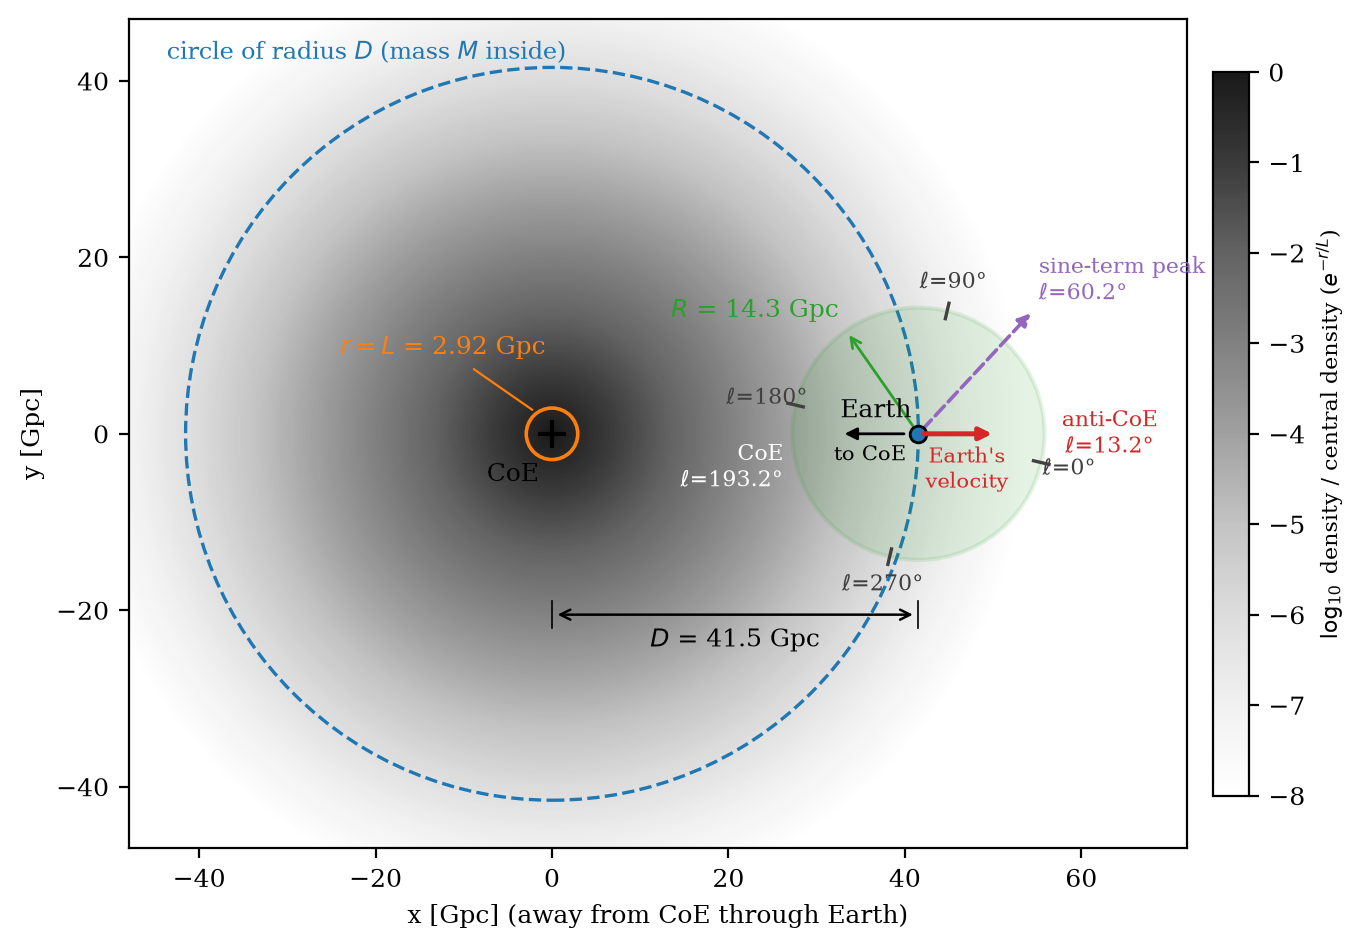
\includegraphics[width=0.97\textwidth]{universe_drawing.png}
\caption{To-scale drawing in the plane of your geometry, in Gpc with equal axes. Grey shading is the $e^{-r/L}$ density on a log scale, the orange circle is $r=L$, and the dashed blue circle of radius $D$ through Earth encloses the mass $M$. The green disc is the vision shell of radius $R$ centred on Earth. Sky directions around Earth are Galactic longitude with $\theta=\ell-\ell_0$, so $\theta=0$ (anti-CoE, $\ell=\ell_0$) points away from the CoE along Earth's velocity. The purple arrow marks the peak of the sine term $1-\mathrm{Amp}\sin(\theta+\varphi)$. The nearest point of the shell lies 9.3 scale lengths from the CoE.}
\end{figure}
\vspace{-8pt}
\noindent\begin{minipage}[t]{0.54\textwidth}\vspace{0pt}\centering
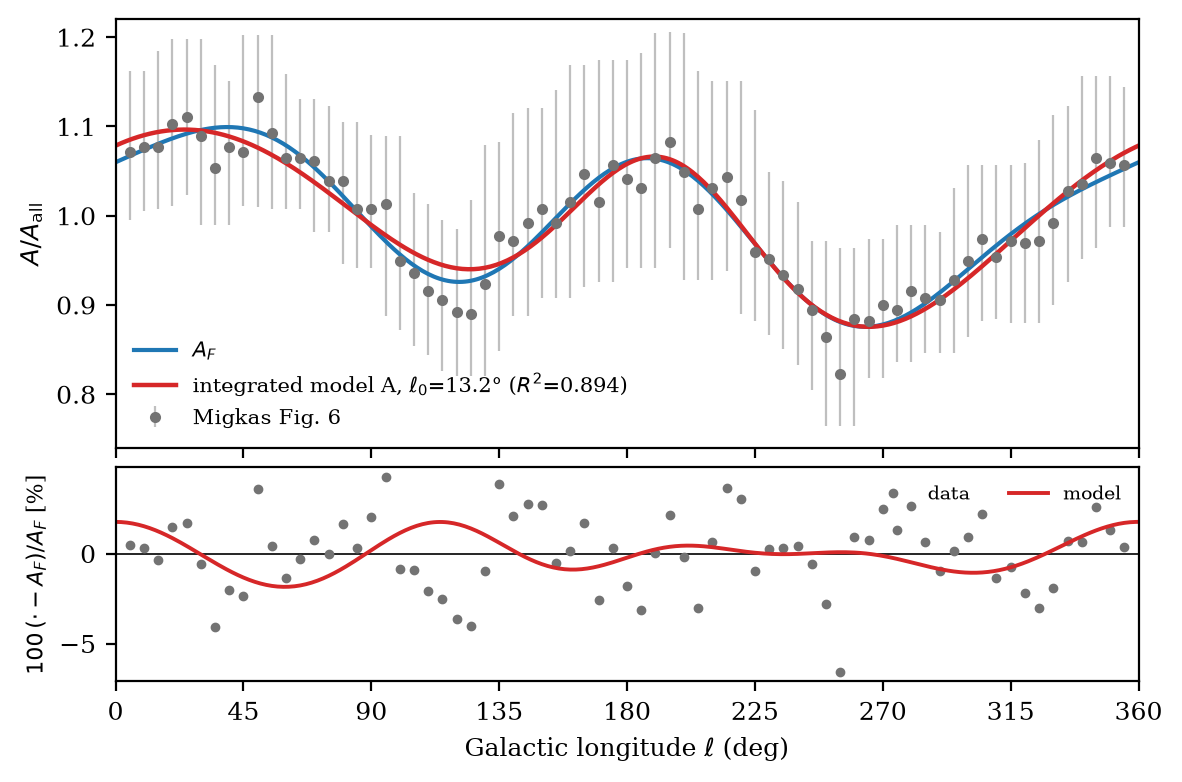
\includegraphics[width=\textwidth]{universe_Achart.png}
\captionof{figure}{Migkas points with error bars, $A_F$, and your model A at the best fit. The lower panel shows data and model as percent differences from $A_F$.}
\end{minipage}\hfill
\begin{minipage}[t]{0.44\textwidth}\vspace{0pt}\centering\scriptsize\setlength{\tabcolsep}{3pt}
\captionof{table}{Best-fit values in your sheet's cells. This $M$ belongs to the integrated model (real $G$, integration from $0.01\,t_0$, profile fixed in space) and does not apply to your one-second kick with $1000\,G$. Milky Way mass taken as $10^{12}\,M_\odot$ including dark matter.}
\begin{tabular}{lll}\toprule
Cell & Quantity & Best fit\\\midrule
C23 & $D/R$ & 2.904\\
D23 & $L/D$ & 0.07028\\
B29 & $R$ & $4.4127\times10^{23}$ km (14.30 Gpc)\\
B28 & $D$ & $1.2816\times10^{24}$ km (41.53 Gpc)\\
B30 & $L$ & $9.007\times10^{22}$ km (2.919 Gpc)\\
B27 & $M$ & $1.944\times10^{54}$ kg\\
    &     & $9.77\times10^{23}\,M_\odot$\\
    &     & $\approx 0.98\times10^{12}$ Milky Ways\\
    & $M/M_{\rm crit}$ ($H_0=70$) & 0.0239\\
BA57 & Amp & $-0.0509$\\
BA59 & $\varphi$ & 0.750 rad\\
 & $\ell_0$ & 13.17$^\circ$\\\midrule
 & $k$ (fixed) & $2.18\times10^{-18}$ s$^{-1}$\\
 & $t_0=1/k$ & 14.5 Gyr\\
 & $G$ (fixed) & $6.674\times10^{-11}$ SI\\
 & $t_i$ (fixed) & $0.01\,t_0$\\\midrule
 & $R^2$ vs 71 Migkas points & 0.894\\
 & $R^2$ vs $A_F$ & 0.979\\\bottomrule
\end{tabular}
\end{minipage}
\end{document}
